\documentclass[10pt,a4paper]{article}
\usepackage[english]{babel}
\usepackage[utf8]{inputenc}
\usepackage{amsmath}
\usepackage{amsfonts}
\usepackage{amssymb}
\usepackage{graphicx}
\usepackage{float}
\usepackage{caption}


\begin{document}
	\part*{Model Documentation of the \\Modular Multilevel Converter}

	%%%%%%%%%%%%%%%%%%%%%% NOMENCLATURE %%%%%%%%%%%%%%%%%%%%%%%%%%%

	\section{Nomenclature}
	\subsection{Nomenclature for Model Equations}
	
	\begin{tabular}{ll}
		$e_{s0}$ & total	stored energy (scaled by $\frac{2}{3}$)\\
		$e_{d0}$ & (vertical)	difference between all upper and all lower arms (scaled by $\frac{2}{3}$)\\
		$\underline{e}_s$ & complex energy sum\\
		$\underline{e}_d$ & complex energy difference\\
		$\theta$ & angle of rotating reference frame of $\underline{e}_s$ and $\underline{e}_d$\\
		$\omega$ & angular speed of the rotating reference frame \\
		$v_{DC}$ & DC voltage of the MMC\\
		$v_{y0}$ & common-mode voltage\\
		$\underline{v}_y$ & complex output voltage\\
		$v_{x0}$ & voltage which drives the DC currents \\
		$\underline{v}_x$ & voltage which drives the internal currents \\		
		$\underline{v}_g$ & grid voltage \\
		$\underline{i}$ & complex output current\\
		$i_{s0}$ & scaled version of DC current \\
		$\underline{i}_s$ & complex circulating current\\
		$L_z$ & arm inductance \\
		$M_z$ & mutual inductance \\
		$R$ & resistance of the load \\
		$L$ & inductance of the load		
	\end{tabular}

	%%%%%%%%%%%%%%%%%%%%%% NOMENCLATURE FOR DERIVATION%%%%%%%%%%%%%%%%%%%%%%%%%%%

	\subsection{Nomenclature for Derivation}
	
	\begin{tabular}{ll}
		$e_{z1}$, ..., $e_{z6}$ & arm energies\\
		$i_{z1}$, ..., $i_{z6}$ & arm currents \\
		$g_0$, $g_\alpha$, $g_\beta$ & clark transform constants \\
		$\underline{g}_{\alpha\beta}$ & complex constant using $g_\alpha$, $g_\beta$ and $\theta$ 
	\end{tabular}
	
	\subsection{Circuit Graphic}	
	\begin{figure}[H]
		\centering
		\captionsetup{justification=centering, margin=1cm}
		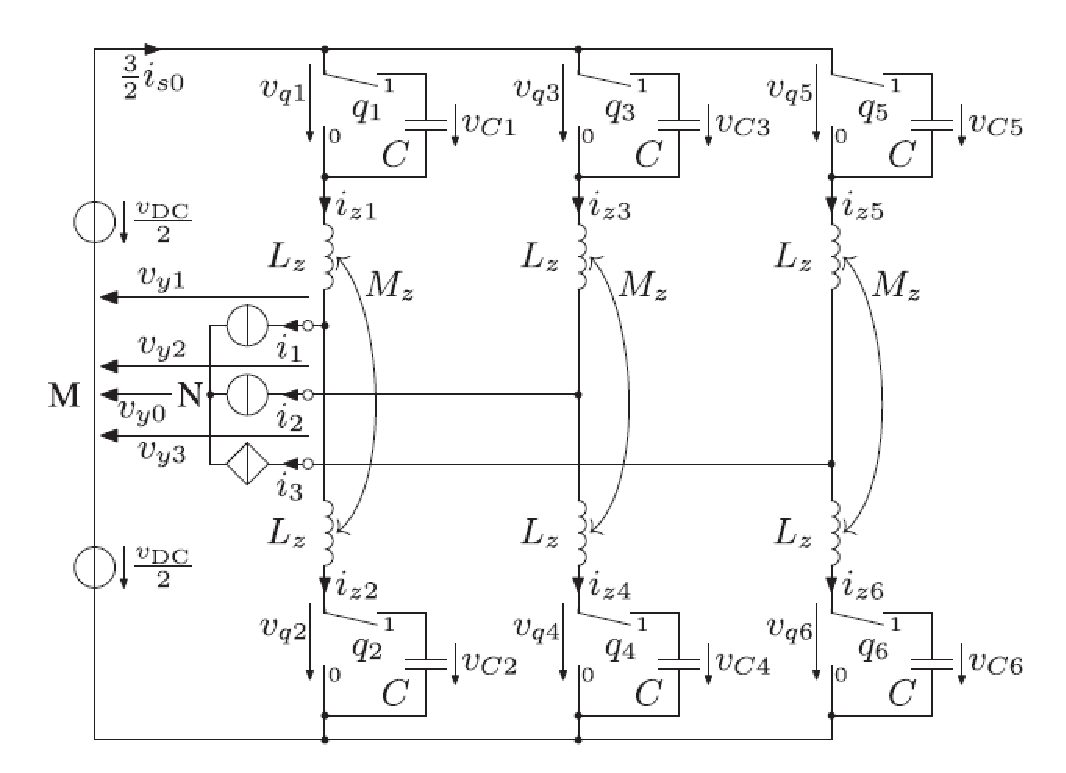
\includegraphics[width=70mm]{mmc.pdf}
		\caption{Circuit. \\ \footnotesize{Source: Fehr, H.; Gensior, A./ Improved Energy Balancing of Grid-Side Modular Multilevel Converters by Optimized Feedforward Circulating Currents and Common-Mode Voltage}}
	\end{figure}

	%%%%%%%%%%%%%%%%%%%%%% MDOEL EQUATIONS %%%%%%%%%%%%%%%%%%%%%%%%%%%
		
	\section{Model Equations}
	
	State Vector and Input Vector:	
	\begin{align*}
		\underline{x} &= (x_1 \ x_2 \ \underline{x}_3 \ \underline{x}_4 \ \underline{x}_5 \ x_6 \ \underline{x}_7 \ x_8)^T = (e_{s0} \ e_{d0} \ \underline{e}_s \ \underline{e}_d \ \underline{i}_s \ i_{s0} \ \underline{i} \ \theta)^T \\
		\underline{u} &= (\underline{u}_1 \ u_2 \ \underline{u}_3 \ u_4)^T = (\underline{v}_y \ v_{y0} \ \underline{v}_x \ v_{x0})^T
	\end{align*}
	
	\noindent Model Equations:	
	\begin{subequations}	
	\begin{align}
		\dot{x}_1 &= v_{DC} \, x_6 - \mathrm{Re} (\underline{x}_7\, \underline{u}_1^*)				\\
		\dot{x}_2 &=-2 u_2\, x_6 - \mathrm{Re} (\underline{x}_5^* \, \underline{v}_{y\Delta})		\\
		\dot{\underline{x}}_3 &=v_{DC}\, \underline{x}_5 - e^{-3j x_8}\, \underline{u}_1^* \, \underline{x}_7^* - 2 \underline{x}_7\, u_2 - j\omega \, \underline{x}_3 		\\
		\dot{\underline{x}}_4 &= v_{DC}\, \underline{x}_7 - e^{-3j x_8}\, \underline{x}_5^* \, \underline{v}_{y\Delta}^* - 2 \underline{x}_5 \, u_2 - 2 x_6\, \underline{v}_{y\Delta} - j\omega \underline{x}_2		 \\
		\dot{\underline{x}_5} &= \frac{1}{L_z+M_z} (\underline{u}_3 - j\omega (L_z+M_z)\, \underline{x}_5 )		\\
		\dot{x_6} &= \frac{1}{L_z+M_z} u_4		\\
		\dot{\underline{x}_7} &= \frac{1}{L} ( \underline{u}_1 - (R+j\omega L)\underline{x}_7 - \underline{v}_g)	\\
		\dot{x}_8 &= \omega
	\end{align}
	\end{subequations}
	with
	
	\begin{align}
		\underline{v}_{y\Delta} &= \underline{u}_1 - M_z (j\omega \underline{i} + \dot{\underline{x}_7})
	\end{align}

	%%%%%%%%%%%%%%%%%%%%%% PARAMETERS | OUTPUTS %%%%%%%%%%%%%%%%%%%%%%%%%%%
	\noindent
	Parameters: $v_{DC}, \ \underline{v}_g, \ \omega, \ L_z, \ M_z, \ R,L$
	\\
	Outputs: $\underline{e}_s, \ e_{s0}, \ \underline{e_d}, \ e_{d0}$
	
	%%%%%%%%%%%%%%%%%%%%%% ASSUMPTIONS %%%%%%%%%%%%%%%%%%%%%%%%%%%	
	
	\subsection{Assumptions}	
	\begin{enumerate}
		\item The cells of the arm $k=$ 1,2,...,6 are represented by one equivalent cell with the duty cycle $q_k \in$ [0,1] and a voltage $v_Ck$ that accords the sum of the individual cells in the arm. This implies that the
		underlying problem of balancing the voltages within each
		arm has already been solved.
		\item The load currents are assumed to be continuous, matched
		to the initial currents of the arm inductors, and satisfy the
		constraint $i_1 + i_2 + i_3 = 0$ caused by junction N.
	\end{enumerate}
	
	%%%%%%%%%%%%%%%%%%%%%% EXEMPLARY PARAMETER VALUES %%%%%%%%%%%%%%%%%%%%%%%%%%%	
	
	\subsection{Exemplary parameter values}
	\begin{tabular}{cl}
\hline
  Symbol  & Value                                                                                                                                                                                \\
\hline
   $A$    & $\left[\begin{matrix}0.8189 & 0.0863 & 0.09 & 0.0813\\0.2524 & 1.0033 & 0.0313 & 0.2004\\-0.0545 & 0.0102 & 0.7901 & -0.258\\-0.1918 & -0.1034 & 0.1602 & 0.8604\end{matrix}\right]$ \\
   $B$    & $\left[\begin{matrix}0.0045 & 0.0044\\0.1001 & 0.01\\0.0003 & -0.0136\\-0.0051 & 0.0936\end{matrix}\right]$                                                                          \\
 $B_{1}$  & $\left[\begin{matrix}0.0045 & 0.0044\\0.1001 & 0.01\\0.0003 & -0.0136\\-0.0051 & 0.0936\end{matrix}\right]$                                                                          \\
 $C_{1}$  & $\left[\begin{matrix}1.0 & 0 & -1.0 & 0\\0 & 0 & 0 & 0\\0 & 0 & 0 & 0\end{matrix}\right]$                                                                                            \\
   $C$    & $\left[\begin{matrix}1.0 & 0 & 0 & 0\\0 & 0 & 1.0 & 0\end{matrix}\right]$                                                                                                            \\
 $D_{11}$ & $\left[\begin{matrix}0 & 0 & 0\\0 & 0 & 0\\0 & 0 & 0\end{matrix}\right]$                                                                                                             \\
 $D_{12}$ & $\left[\begin{matrix}0 & 0\\1.0 & 0\\0 & 1.0\end{matrix}\right]$                                                                                                                     \\
 $D_{21}$ & $\left[\begin{matrix}0 & 1.0 & 0\\0 & 0 & 1.0\end{matrix}\right]$                                                                                                                    \\
\hline
\end{tabular}

	%%%%%%%%%%%%%%%%%%%%%% DERIVATION & EXPLANATION %%%%%%%%%%%%%%%%%%%%%%%%%%%	
			
	\section{Derivation and Explanation} 
	The six arm energies $e_{z1}$, ..., $e_{z6}$ transformed into  
	\begin{subequations}	
	\begin{align}
		e_{s0} &= 2g_0 \, [(e_{z1},e_{z3},e_{z5})^T+(e_{z2},e_{z4},e_{z6})^T] 	\\
		e_{d0} &=2g_0 \, [(e_{z1},e_{z3},e_{z5})^T-(e_{z2},e_{z4},e_{z6})^T]	\\
		\underline{e}_s &=2\underline{g}_{\alpha\beta} \, [(e_{z1},e_{z3},e_{z5})^T+(e_{z2},e_{z4},e_{z6})^T]	\\
		\underline{e}_d &=2\underline{g}_{\alpha\beta} \, [(e_{z1},e_{z3},e_{z5})^T-(e_{z2},e_{z4},e_{z6})^T]
	\end{align}	
	\end{subequations}
	with use of the Clark Transform
	
	\begin{equation}
		T_{0\alpha\beta}= \frac{1}{3} 
		\left(\begin{array}{rrr}
			1 & 1 & 1\\
			2 & -1 & -1 \\
			0 & \sqrt{3} & -\sqrt{3}
		\end{array} \right) = 
		\left( \begin{array}{r}
			g_0 \\ g_\alpha \\ g_\beta
		\end{array}\right)
	\end{equation}
	and $\underline{g}_{\alpha\beta}=e^{-j\theta}(g_{\alpha}+jg_{\beta})$. \\
	The currents can be transformed as
	\begin{subequations}
	\begin{align}
		i_{s0} &= 2g_0 \, [(i_{z1},i_{z3},i_{z5})^T+(i_{z2},i_{z4},i_{z6})^T]	\\
		0 &= g_0 (i_1,i_2,i_3)^T 	\\
		\underline{i}_s &= \underline{g}_{\alpha\beta} \, [(i_{z1},i_{z3},i_{z5})^T+(i_{z2},i_{z4},i_{z6})^T]	\\
		\underline{i} &= \underline{g}_{\alpha\beta} \, (i_1,i_2,i_3)^T.
	\end{align}	
	\end{subequations}
	The voltages are transformed as
	\begin{subequations}	
	\begin{align}
		v_{x0} &= g_0 \, [v_{DC}(1,1,1)^T - (v_{q1},v_{q3},v_{q5})^T-(v_{q2},v_{4},v_{q6})^T]		\\
		v_{y0} &= g_0 \, (v_{y1},v_{y2},v_{y3})^T 	\\
		\underline{v}_x &= \underline{g}_{\alpha\beta} \, [v_{DC}(1,1,1)^T - (v_{q1},v_{q3},v_{q5})^T-(v_{q2},v_{4},v_{q6})^T]		\\
		\underline{v}_y &= \underline{g}_{\alpha\beta} \, (v_{y1},v_{y2},v_{y3})^T \\
		&= \underline{g}_{\alpha\beta} \, [(v_{q2},v_{4},v_{q6})^T - (v_{q1},v_{q3},v_{q5})^T - (L_z - M_z) \frac{d}{dt}(i_1,i_2,i_3)^T ].
	\end{align}
	\end{subequations}
	
	%%%%%%%%%%%%%%%%%%%%%% REFERENCES %%%%%%%%%%%%%%%%%%%%%%%%%%%
	


	\begin{thebibliography}{10}		
		\bibitem{FG18}Fehr, H.; Gensior, A.: 
		\textit{Improved Energy Balancing of Grid-Side Modular
			Multilevel Converters by Optimized Feedforward
			Circulating Currents and Common-Mode Voltage}, IEEE 2018.
	\end{thebibliography}

\end{document}

